\documentclass[../main.tex]{subfiles}

\begin{document}

\renewcommand{\labelitemi}{\ding{226}}
\renewcommand{\labelitemii}{\ding{227}}

\chapter{The T2K experiment}
\label{part:T2K:general}

The T2K (Tokai to Kamioka) is a long-baseline accelerator neutrino experiment. Its main propose is precise measurements of the neutrino oscillation parameters. T2K is a continuation of the successful history of the previous accelerator experiments: KEK, MINOS, etc. At the beginning of the T2K era, the main goal was the measurements of the $\theta_{13}$ mixing angle. At that moment its value was not measured at all and $\theta{13}=0$ was possible. The value of this angle is important as the amplitude of the CP--violation (\autoref{sec:intro:cp} of \autoref{ch:nu_phys}) is scaled with $\theta_{13}$. Even with the maximum value of the $\delta_{CP}$ the effect could vanish with zero mixing angle. Thus $\theta_{13}$ became the main goal at the beginning of the T2K era.

The concept of the experiment is the following:
\begin{enumerate}
  \item 30 $GeV/c^2$ proton beam produced with the J-PARC accelerator hits the carbon target producing mesons. At these energies mainly pions and kaons are born.
  \item The mesons are focused with three horns into the decay volume. The horn polarity defines whether positive or negative mesons will be focused.
  \item In the decay volume the mesons decay mostly into the muon neutrino or anti-neutrino. Thus the horn polarity defines the neutrino mode ($H\to\mu^+\nu_{\mu}$ or $\overline{H}\to\mu^-\overline{\nu}_{\mu}$). The energy spectrum of the off-axis neutrino beam is quasi-monoenergetic peaking around 0.6 GeV.
  \item The non-oscillated neutrino beam is studied with the near detector complex: on-axis INGRID and off-axis ND280 (\autoref{ch:T2K:nd})
  \item After traveling 295 km neutrino beam fix the far detector complex Super-Kamiokande (\autoref{ch:T2K:sk}). The baseline and neutrino energy are tuned to the first oscillation maximum ($\Delta m ^2_{32}L/E\approx1$).
\end{enumerate}

The main goals of the T2K experiment are:
\begin{itemize}
  \item precise measurements of the oscillation parameters $\Delta m^2_{23}$ and $\theta_{23}$ with the muon neutrino disappearance $\nu_\mu\to\nu_\mu$ and $\overline{\nu}_\mu\to\overline{\nu}_\mu$
  \item measurements of the  $\theta_{13}$ with the electron appearance $\nu_\mu\to\nu_e$ and $\overline{\nu}_\mu\to\overline{\nu}_e$
  \item search for the CP violation $sin\delta_{CP}\neq0$ with studying the difference between $\nu_\mu\to\nu_e$ and $\overline{\nu}_\mu\to\overline{\nu}_e$
  \item along with the oscillation measurements the neutrino interactions are studied carefully in order to reduce the systematic uncertainty. Thus the neutrino cross-sections on carbon, water and iron.
\end{itemize}

Alongside reactor experiments T2K successfully measured the non-zero value of the $\theta_{13}$ thus opening the way for the CP--violation search. At the moment it's a major goal of the experiment together with more precise measurements of other oscillation parameters. In this chapter the details about the T2K setup as well as an analysis technique will be overviewed.

\section{Neutrino beam}
\label{ch:T2K:nu_beam}

In order to perform the precise measurements of the neutrino oscillation parameters accurate knowledge about the initial neutrino beam is essential. Accelerator experiments are able to use the benefits of the well-known and controlled man-made neutrino beam to reduce the uncertainty of the measurements. In this section the details about the beam production and monitoring within the T2K experiment will be presented.
\subsection{General concept}
The T2K experiment use so-called ``off-axis'' concept to obtain quasi-monoenergetic neutrino beam. The dominating neutrino production mode in the T2K is pion decay $\pi\to\mu\nu$. The neutrino energy in the two-body decay will be given by
\begin{equation}
E_\nu\approx\left(1-\frac{m_\mu^2}{m_\pi^2}\right)\frac{E_\pi}{1+\gamma^2\theta^2}
\end{equation}

where $\gamma$ is the pion kinematic parameter ant $\theta$ is a neutrino direction angle w.r.t. pion momentum. The equality of the derivative of the neutrino energy over the pion energy to zero means full independence of the first from the latter. In case $\theta=\gamma^{-1}$ $dE_\nu/dE_\pi=0$ that means that neutrino energy depends weakly on the parent pion energy. Finally we will get
\begin{equation}
E_\nu\approx\left(1-\frac{m_\mu^2}{m_\pi^2}\right)\frac{m_\pi}{2\theta}\approx\frac{29.8MeV}{\theta}
\end{equation}

The T2K beamline allows varying of the peak neutrino energy by tuning the off-axis angle. The energy spectra for different angles are provided in \autoref{fig:t2k:nu_beam_oa}. The figure provides also the oscillation probability of the muon neutrino at the distance of 295 km versus the energy. Thus with the off-axis angle tuning the maximum oscillation effect could be measured.
\begin{figure}[!ht]
  \centering
  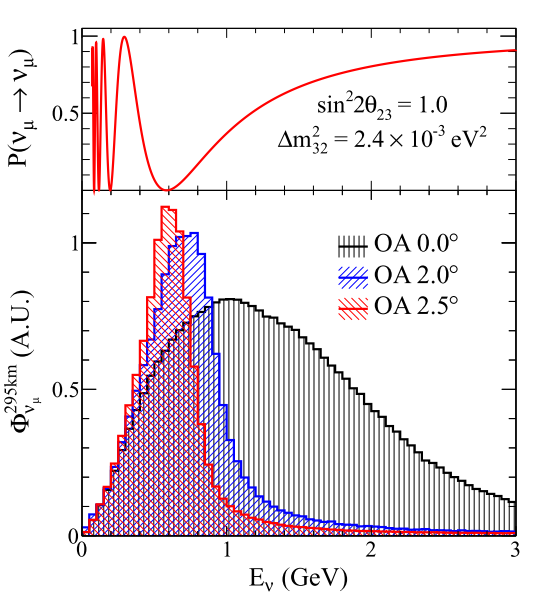
\includegraphics[width=0.5\linewidth]{nu_beam}
  \caption{Muon neutrino survival probability at 295 km and neutrino fluxes for different off-axis angles. Figure from~\cite{Abe2013}.}
  \label{fig:t2k:nu_beam_oa}
\end{figure}

\subsection{Neutrino beamline}
The T2K neutrino beamline could be generally divided into two stages: primary beamline and secondary beamline. The first takes the protons from the J-PARC accelerator main ring, performs measurements of the beam parameters and focuses it on a carbon target. The secondary beamline focuses the produced mesons with the horns into the decay volume and monitor its decay. The general scheme of the beamline is shown in \autoref{fig:t2k:beamline}. The detailed description could be found in~\cite{Abe2013}.

\begin{figure}[!ht]
  \centering
  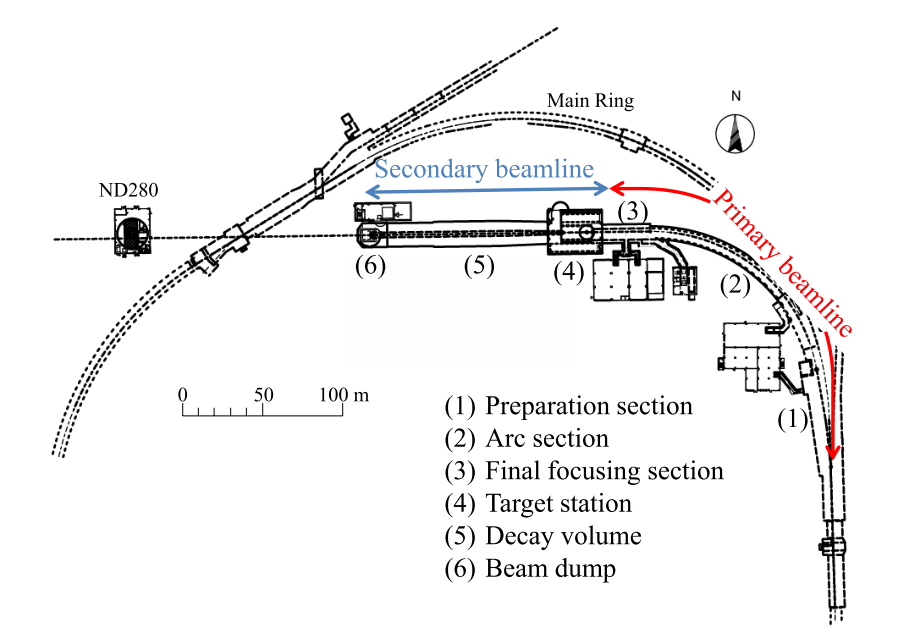
\includegraphics[width=0.7\linewidth]{beamline}
  \caption{The scheme of the T2K neutrino beam line. Primary beamline (proton line) is shown in red and secondary beamline is shown in blue.}
  \label{fig:t2k:beamline}
\end{figure}

\subsubsection{Primary beamline}
The primary beamline takes the proton from the J-PARC main ring. The beam is structured into the spills coming with 0.5 Hz rate. Each spill is 5 $\mu s$ wide and consists of 8 bunches with $\sigma\approx18 ns$ and 58 ns separation. Per each spill $3\times10^{14}$ protons could be delivered. Thus the total maximum power of the beamline could be estimated as 750 kW. The total number of protons hit into the target is used as a main characteristic of the statistics collected in T2K experiment (POT - Protons On Target). The evolution of the accumulated statistics as well as the beam power is shown in \autoref{fig:t2k:POT}.

\begin{figure}[!ht]
  \centering
  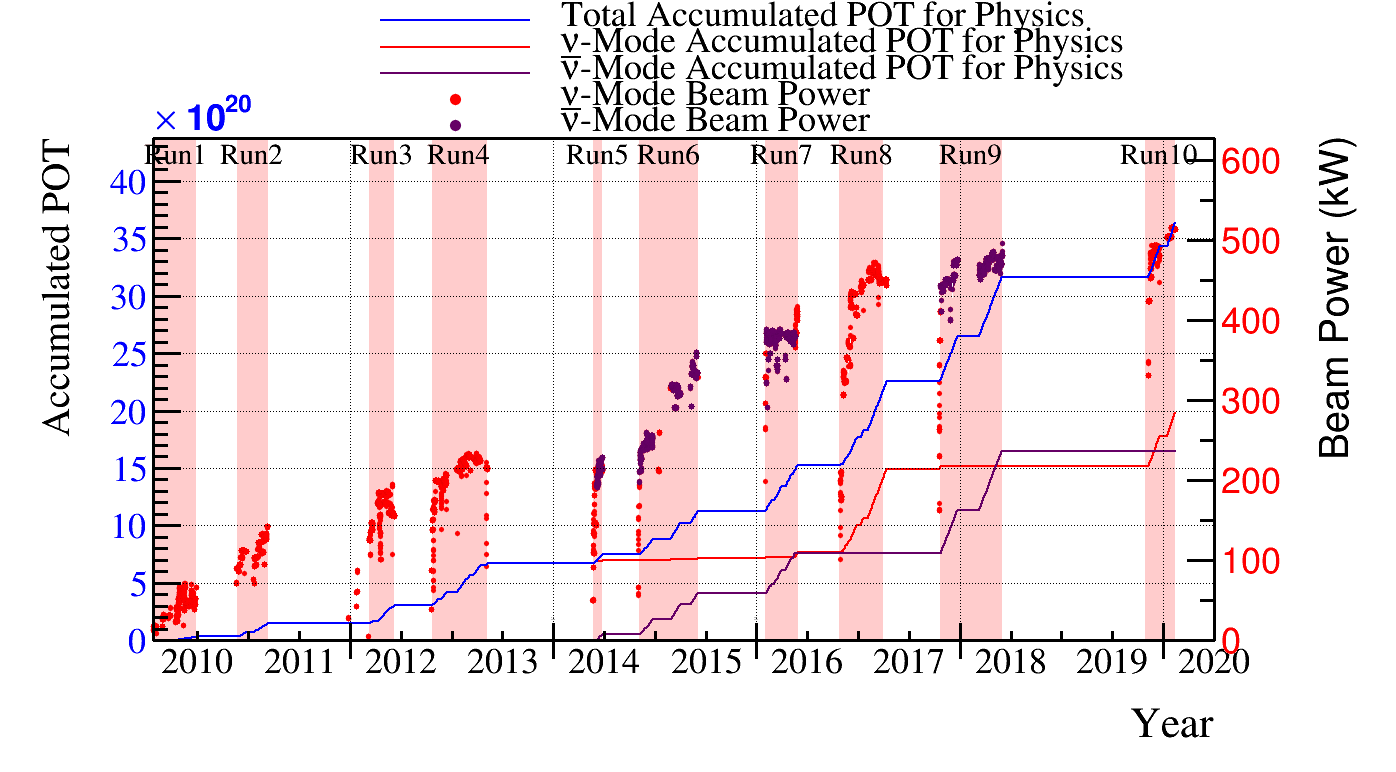
\includegraphics[width=0.7\linewidth]{POT}
  \caption{The collected statistics in the T2K experiment in POT (Proton On Target) together with the beam intensity along the data accumulation.}
  \label{fig:t2k:POT}
\end{figure}

The initial beam is bounded with the arc section made with superconducting magnets and horizontally aligned with the direction to the detectors. At this stage the measurements of the beam parameters are performed. The beam intensity is measured with current transformers that use toroidal coils around a cylindrical ferromagnetic core. The uncertainties of the measurements are estimated at the level of 2\%. The beam position is measured with electrostatic monitors and secondary emission monitors. First measures the beam position with the accuracy of 450 $\mu m$ the latter measures the beam width with the precision 200 $\mu m$. After the measurements the beam is directed downward and focused on the carbon target.

\subsubsection{Secondary beamline}
The secondary beamline is responsible for neutrino production. The target for protons is made of Carbon cylinder 2.6 cm width and 91.4 cm length (1.9 interaction length). During the irradiation target heats up to 800$^\circ$C. The core is put with the titanium case for fast heat transfer to the water cooling system. The target is inserted into the first magnetic horn, so the mesons are affected by the focusing magnetic field from the moment of production.

The meson focusing system consists of three magnetic horns. The first one contains the target where the mesons are produced. The horns are operated with the pulsed current at the level of 250-320 kA. The polarity could be changed in order to focus negative or positive mesons resulting in neutrino or anti-neutrino production. The dramatic gain of the horn usage for the neutrino beam intensity is shown in \autoref{fig:t2k:horn}.

The hadrons are focused into the decay volume. It's a 96 m tunnel widening from 1.4x1.7 $m^2$ at the beginning up to the 3.0x5.0 $m^2$ at the end. The volume is filled with argon gas and is cooled with water. The parent particles are considered as possible neutron sources are $\pi^\pm$, $K^\pm$, $K^0_L$ and $\mu^\pm$. The most probable neutrino production reactions are:
\begin{align}
\pi^\mp&\to\mu^\mp\overset{\scriptscriptstyle(-)}{\nu_\mu} \hspace{2cm} &K^\mp\to\mu^\mp\overset{\scriptscriptstyle(-)}{\nu_\mu} \\
K^\mp&\to\pi^0e^\mp\overset{\scriptscriptstyle(-)}{\nu_e} \hspace{2cm}  &\mu^\mp\to e^\mp\overset{\scriptscriptstyle(-)}{\nu_\mu}\overset{\scriptscriptstyle(-)}{\nu_e}
\end{align}

The energy spectra divided into neutrino flavor and parent particle are provided in \autoref{fig:t2k:nu_beam}.

\begin{figure}[!ht]
  \centering
  \begin{minipage}{0.32\linewidth}
    \centering
    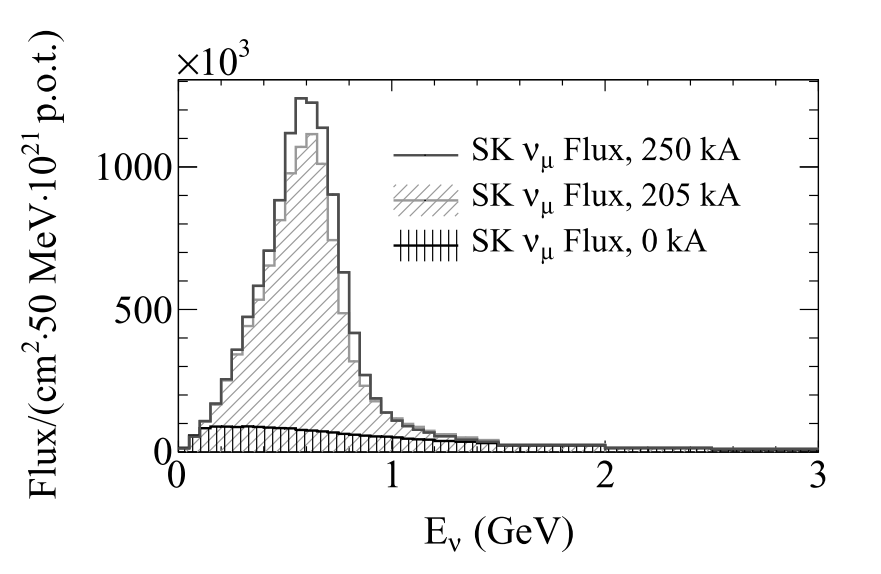
\includegraphics[width=\linewidth]{horn}
    \caption{The effect of horn usage on the beam intensity at the far detector}
    \label{fig:t2k:horn}
  \end{minipage}
  \begin{minipage}{0.66\linewidth}
    \centering
    \begin{minipage}{0.49\linewidth}
    \centering
      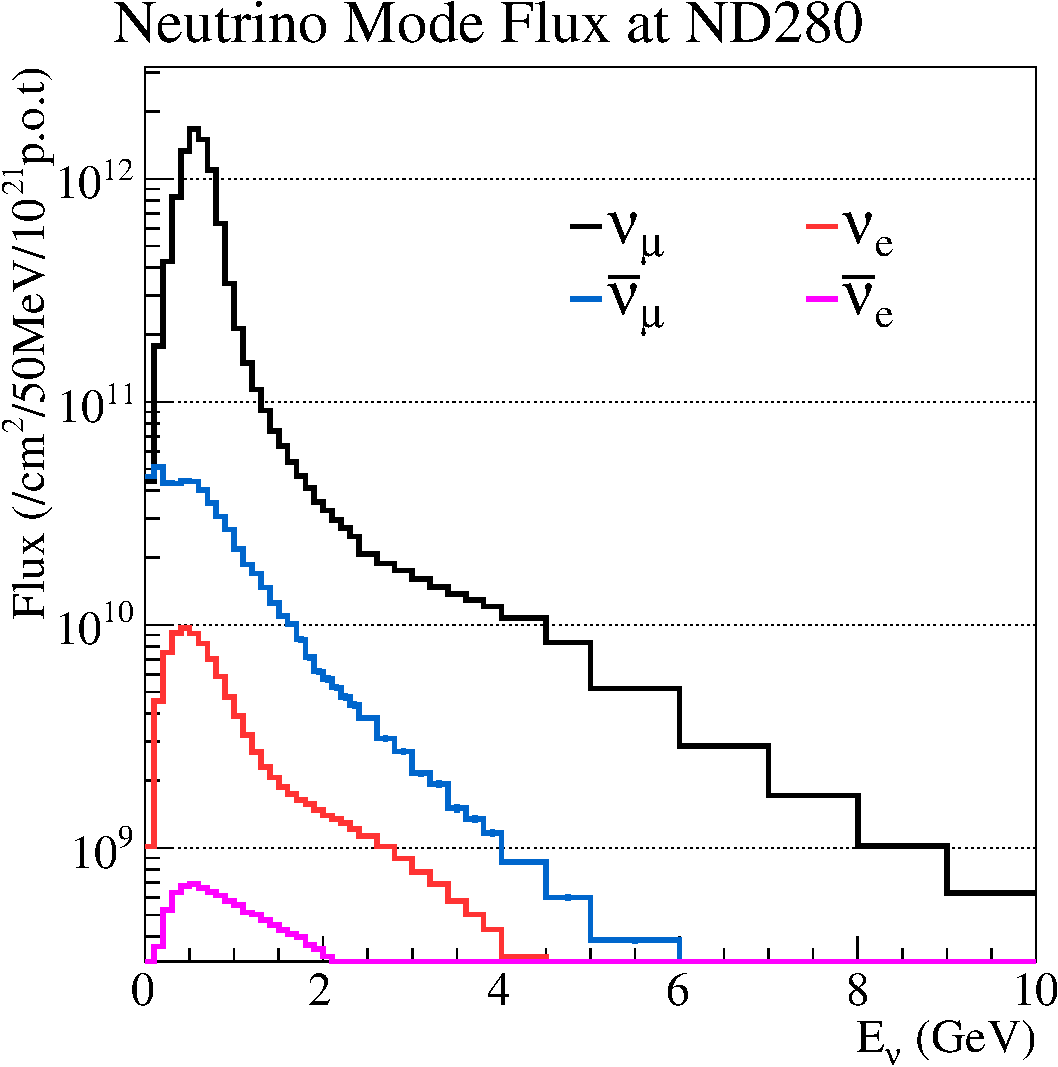
\includegraphics[width=\linewidth]{nu_flux_flavor} \\ (a)
    \end{minipage}
    \begin{minipage}{0.49\linewidth}
    \centering
      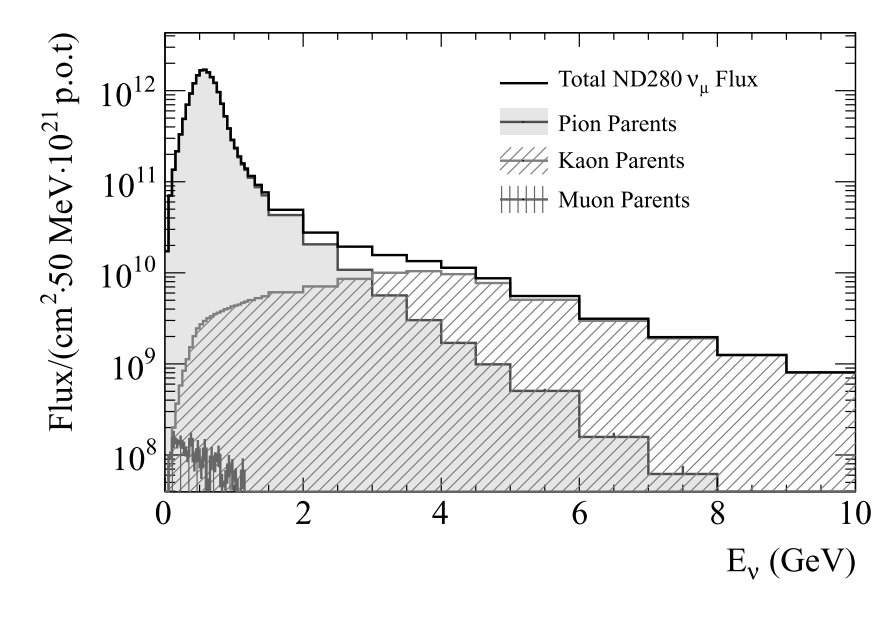
\includegraphics[width=\linewidth]{nu_flux_parent} \\ (b)
    \end{minipage}
    \caption{The neutrino beam at the near detector side divided into (a) neutrino flavor and (b) parent particle.}
    \label{fig:t2k:nu_beam}
  \end{minipage}
\end{figure}

Just after the decay pipe the beam dump is placed. It's made of 75 tons of graphite and the main goal is to suppress the charge particle beam +as much as possible. Thus mesons will interact in the dump and will not produce neutrino behind the decay volume. Such neutrinos will have the different off-axis angle and will not have the proper energy, that's why the meson beam should be stopped. Though muons with high energies (> 5 GeV) could go through the beam dump. They are used to measure the stability of the neutrino beam. Muons are produced in the hadron decays along with neutrino, thus the muon spectrum fluctuation will explicitly indicate the fluctuation of the neutrino beam.

\section{Near detector}
\label{ch:T2K:nd}
Precise knowledge about the initial neutrino beam is essential for the accurate oscillation measurements. The T2K near detector complex is placed in 280 meters from the proton target and its main goal is the monitoring of the unoscillated beam. Two detectors are used for this propose: on-axis INGRID and off-axis ND280. The schematic views of both detectors are presented in \autoref{fig:T2K:ND280}.

\begin{figure}[!ht]
  \centering
  \begin{minipage}{0.49\linewidth}
    \centering
    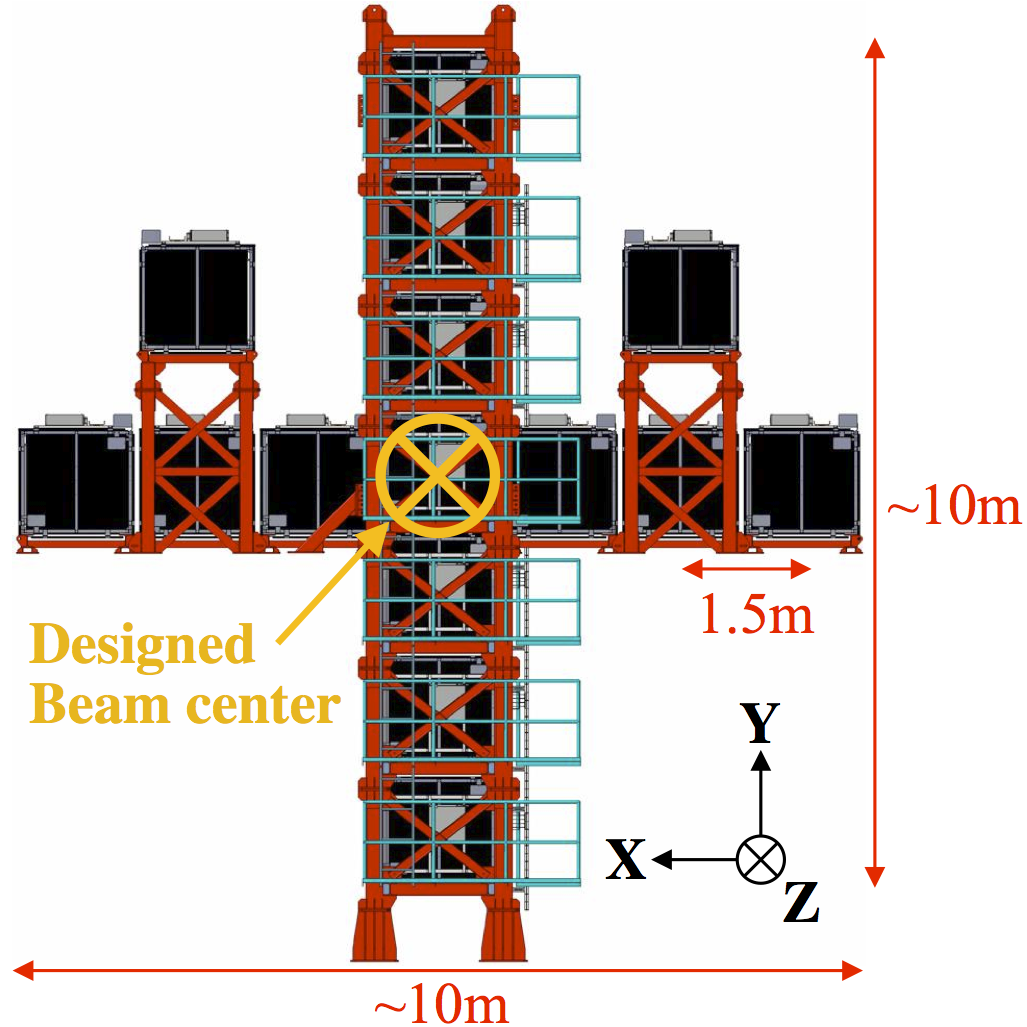
\includegraphics[width = \linewidth]{INGRID} \\ (a)
  \end{minipage}
  \begin{minipage}{0.49\linewidth}
    \centering
    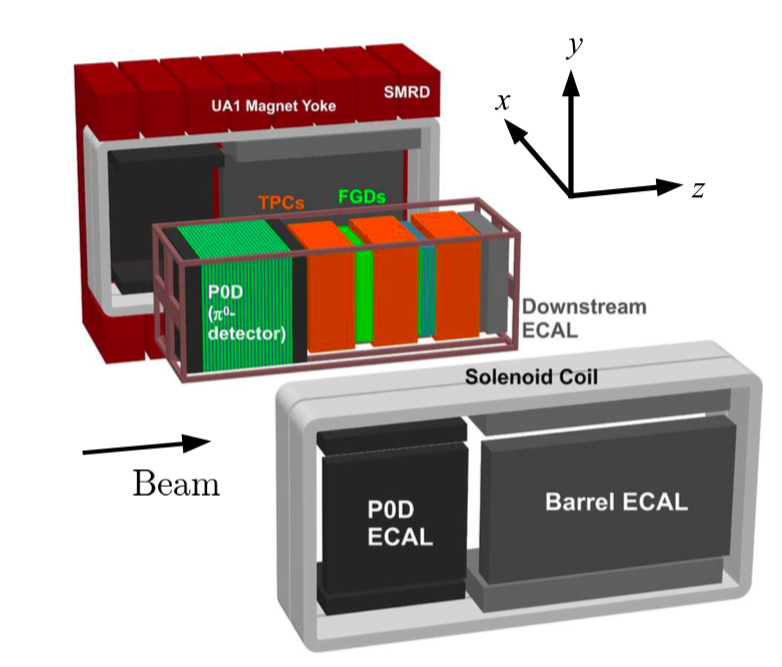
\includegraphics[width = \linewidth]{ND280} \\ (b)
  \end{minipage}
    \caption{An exploded view of the near detector complex: (a) on-axis INGRID detector, (b) off-axis ND280 detector.}
    \label{fig:T2K:ND280}
\end{figure}

\subsection {INGRID}
The main goal of the INGRID detector is controlling the position and intensity of the neutrino beam. It consists of 14 modules arranged in a cross with two additional modules placed outside the main cross (\autoref{fig:T2K:ND280} (a)). The center of the cross is placed at 0$^\circ$ angle w.r.t. proton beam direction. Each detector module consists of sandwich of iron and tracking planes. With the T2K intensities we expect enough neutrino interactions in the iron targets everyday for the day-to-day monitoring of the neutrino beam parameters. The \autoref{fig:t2k:ingrid_beam} represent the results of such measurements. Both intensity and direction variations are small and the resulting uncertainty in the oscillation analysis is far from dominating.

\begin{figure}{!ht}
  \centering
  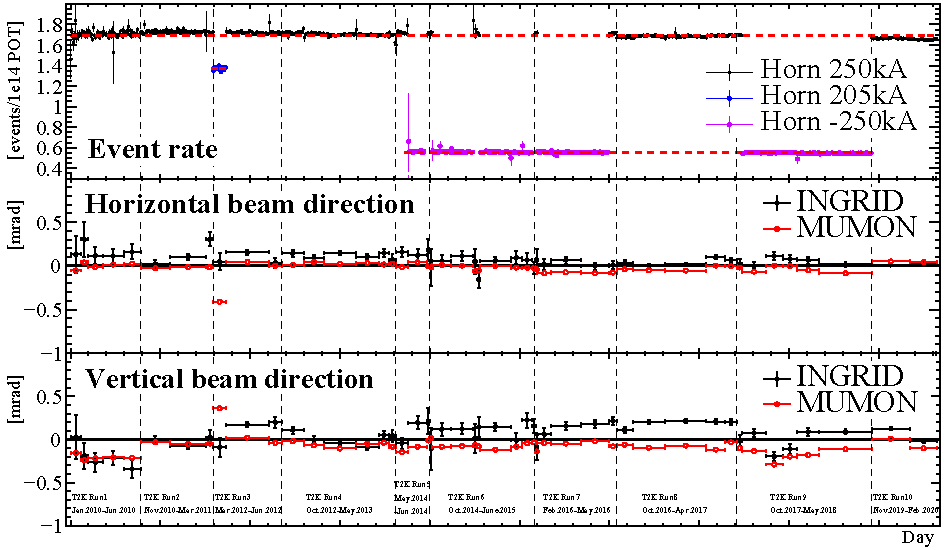
\includegraphics[width=0.8\linewidth]{ingrid_beam}
  \caption{The INGRID measurements of the neutrino beam intensity and position.}
  \label{fig:t2k:ingrid_beam}
\end{figure}

\subsection{Near detector ND280}
\label{sec:T2K:nd280}
The ND280 is an off-axis detector placed at the direction from the target towards the far detector Super-Kamiokande. Its goal is neutrino interaction measurements dividing them into neutrino sign, flavor and the reaction topology. For this propose the detector is composed of plenty of different sub-detectors. The Fine Grained Detectors (FGD) are used as a target for neutrino interaction and the tracking of the outgoing particles. The Time Projection Chambers (TPC) are used for particle identification with the ionization energy loss. Also they help with the momentum reconstruction of the track with its curvature in the magnetic field. Electromagnetic calorimeter (ECAL) detect the gamma conversion and improve electron and muon separation. The SMRD detector works as a trigger for the cosmic rays and may help with the muon identification. The P0D detector is used for the measurements of the $\pi^0$ production in the neutrino interactions. At the beginning of the T2K it was a big concern about the neutral pion production as the main background for the far detector. The $\pi^0$ could be produced in the neutrino interactions and decays mainly into two photons. The photons at these energies are mostly subject to conversion into electron-positron pair. With the water Cherenkov detector we could easily confuse such an event with the single electron production indicating the rare process of electron neutrino appearance --- the main subject of the T2K experiment. That's why the precise measurements of the $\pi^0$ production with the near detector were required.

The ND280 measurements are used to constrain the parameters of the flux and the theoretical models of the neutrino interactions. The fact that we have knowledge about the neutrino sign, flavor and reaction type allows us to probe plenty of the models' parameters independently. This will result in the smaller uncertainty of the global oscillation analysis. In the following subsections the subdetectors structure and features will be overviewed.

\subsubsection{Fine grained detectors (FGD)}
Two FGD modules~\cite{Amaudruz2012} are used as a target for the neutrino interactions. The size of the module is 2x2x0.3 $m^3$. They consists of sandwich structure of bars made with plastic scintillators and oriented along X and Y axis, while beam is coming along Z axis. The bars are pierced with wavelength shifting fibers (WLS) for the light collection and transportation to the photosensors. The light readout is done with multi-pixel photo counters (MPPC) that provide high detection efficiency and sufficient dynamic range.

In the second FGD the plastic layers are alternated with the water modules. Thus the measurements of the neutrino interaction with the water could be done. In the context of T2K such a measurement is important as far detector uses water target only. The difference between neutrino interaction cross-section with Carbon and Oxygen could be a source of systematic uncertainty.

\subsubsection{Time projection chambers (TPC)}
The TPCs~\cite{Abgrall2011} are gaseous detectors that perform the 3D reconstruction of the charged particle's track. The scheme of the detector is presented in \autoref{fig:t2k:tpc}.

\begin{figure}[!ht]
  \centering
  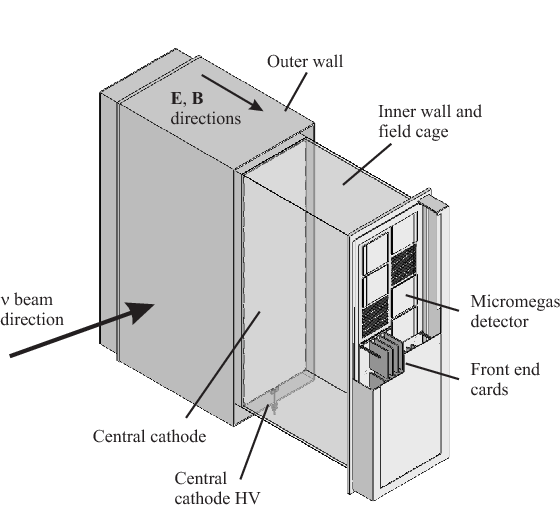
\includegraphics[width=0.6\linewidth]{tpc}
  \caption{The scheme of the TPC module}
  \label{fig:t2k:tpc}
\end{figure}

The general principle of the TPC operation and the key characteristics of the T2K TPCs are presented in \autoref{fig:t2k:tpc_p}. The active volume of the detector is filled with the gas mixture of Argon, $CF_4$ (tetrafluoromethane) and $iC_4H_{10}$ (isobutane) in the volume proportions 95:3:2. A charged particle going through the gas volume it loses the energy through the ionization. The electrons from the ionization drift against the direction of the electric field - from the cathode towards the MicroMegas. The positive ions are drifting towards the cathode. The Argon was chosen as a main component of the gas mixture because a noble gas will minimize the secondary interactions and transport the electrons with minimum distortions. Isobutane also serves for the higher precision of the measurements absorbing photons emitted in the gas thus preventing secondary avalanches. $CF_4$ is responsible for the electron drift speed slow down.

\begin{figure}[!ht]
  \centering
  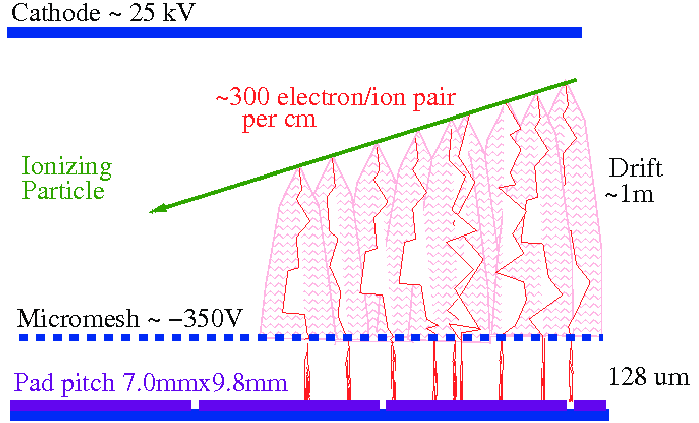
\includegraphics[width=0.5\linewidth]{TPC_principe}
  \caption{The general concept of the TPC operation.}
  \label{fig:t2k:tpc_p}
\end{figure}

The electric field strength is constant in the drift region, ideally there should be no amplification there. The voltage between the cathode and micro mesh is 25 kV at a distance of ~1 meter. At the micro mesh the signal is dramatically amplified as the voltage 350 V is applied for the 128 $\mu m$ gap. The resulting avalanches are detected with the 6.9x9.7 $mm^2$ pads. Here the electrons are transformed into the analog signal that will be later digitized with the electronics.

In total the readout surface of one TPC module consists of 12 MicroMegas 48x36 pads each. For each track the 2D projection (YZ) could be easily reconstructed with the hit pads. The X coordinate depends on the electron drift time. Though the time delay from different parts of the is measured precisely this is an arbitrary measurement. The track curvature in XY plane is known but for the absolute position the external detector (FGD) is essential.

The core of the ND280 - the tracker, consists of 3 TPCs alternated with 2 FGDs. Such a structure is aimed for the effective detection of the lepton produced in the neutrino interactions inside FGDs.

\subsubsection{Electromagnetic calorimeter (ECaL)}
The calorimeters are used for the detection of the gammas from the $pi^0$, produced in the neutrino interactions. They also could help with the particle identification as electrons and hadrons will produce showers while muons will have a clear clean track. The calorimeters are surrounding the inner detectors of the ND280. They consists of the sandwich structure of plastic bars 4x1 $cm^2$ in cross section, alternating with 1.75 mm thick absorber layers made with lead. The downstream ECaL consists of 34 layers and provide the most precise results, while P0D and barrel ECaL consists of 31 layers.

\subsubsection{Side muon range detector (SMRD)}
The SMRD is surrounding the whole ND280 and is a multifunction detector. It could eject the events triggered by the cosmic rays or the neutrino interactions in the outer detectors or concrete of the pit. SMRD is useful for detection of the muons that exit the detector with high angles. Since there is no TPC at this direction the momentum measurement could be done only with SMRD. The detector itself consists of 440 1.7 cm thick plastic scintillator modules that are inserted in the gaps between 4.8 thick steel plates of the magnet yoke.


\section{SuperKamiokande}
\label{ch:T2K:sk}
The far detector of the T2K experiment is Super-Kamiokande (SK) located 295 km away from the proton target in the Kamioka mine under the Ikenoyama mountain. 50 tons of water are used as a target for the neutrino. The water tank is viewed by 13 thousand of the photomultipliers (PMT) aimed the detection of the Cherenkov light from the charged lepton produced in the neutrino interactions. The schematic view of the detector is presented in \autoref{fig:t2k:sk}.

\begin{figure}[!ht]
  \centering
  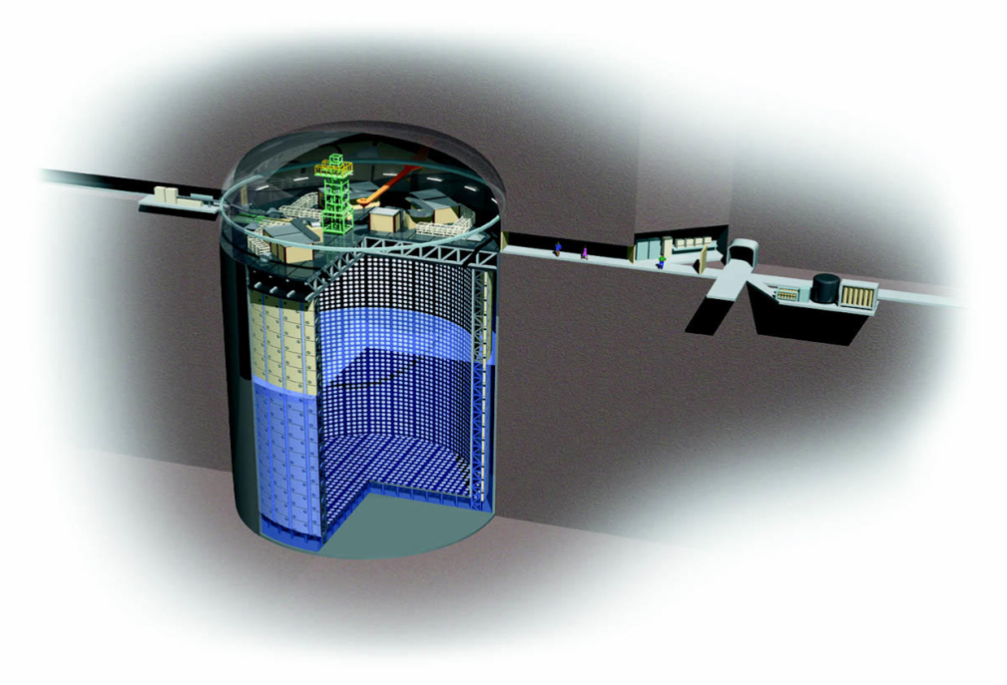
\includegraphics[width=0.7\linewidth]{sk_tank}
  \caption{The scheme of the Super-Kamiokande detector.}
  \label{fig:t2k:sk}
\end{figure}

The working principle of the detector is based on the effect of Cherenkov radiation. When a charged particle passes through a dielectric medium at a speed greater than the phase velocity of light in that medium the conic wave front in formed. The opening angle of the cone is defined by the particle speed and the refraction coefficient of the medium $\cos{\theta}=1/n\beta$, where $\beta=v/c$. The emission of the radiation in a threshold effect. As could be seen from the equation above, the wavefront could be formed only if the particle is fast enough $\beta>1/n$. For the water detector the thresholds are: 1.4 GeV for protons, 160 MeV for muons and 775 keV for electrons. The maximum angle is also limited by $\theta_{max}=arccos(1/n)\approx42^\circ$.

Super-Kamiokande continues the successful history of the neutrino detectors in the Kamioka mine. The first experiment KamiokaNDE (Kamioka Nucleon Decay experiment) started looking for the nucleon decays in 1983. The neutrino interactions were supposed to be the main background. During the detector operation nice performance of the neutrino detection was observed and the experiment was refocused on the neutrino analysis. Since then the detector was massively improved, new setups were build: Kamiokande II, Super-Kamiokande. The latter is operating now as a far detector of the T2K experiment. The ultimate experience collected during the studies in Kamioka allows the excellent physics performance.

There are many challenges in neutrino studies with water Cherenkov detectors. First of all, due to the small cross-section the statistics is limited. In order to increase the number of events the detector was enlarged several times from 3 kt (KamiokaNDE) to 50 kt (Super-Kamiokande). With the larger tank the detection of the Cherenkov light becomes as issue. The intensity of such a light is quite low. Resulting the hard work of the SK collaboration the water purity is remaining extremely high keeping the transparency at the level of 100 meters. The other issue is photon detection itself. The photo coverage of the active area surface is 40\% aiming to collect as much photons as possible. Large 20-inch PMT with high detection efficiency are used for it. The wavelength of the Cherenkov light is tending to the ultraviolet region, while the efficiency of the photocathods is quite low in this region. The light intensity decreased as $\lambda^3$ with the increasing of the wavelength, that's why the excellent performance of the PMT is essential for the successful detector operation.

The other challenge is a background suppression. The detector is placed in mine in order to reduce the flux of the cosmic rays. Though extremely high muons could reach the water tank. The SuperKamiokande is divided into two volumes: inner and outer detectors. There isolated for the light, so the detection of the light in the outer volume will explicitly indicate the out of tank particle production. For the neutrino analysis only leptons produced in the inner detector are considered. For safety the active volume is reduced with 2m tolerance from each wall reducing the fiducial volume to 22.5 tons.

The detector allows separating Cherenkov ring produced by muon and electron. Due to lighter mass electrons are more subject to breaking radiation. Since the critical energy for the electrons in water is tens MeV and the typical electrons energy produced by the T2K neutrinos is hundreds MeV, we expect to see electromagnetic showers that will distort the Cherenkov ring. The examples of the events are presented in \autoref{fig:T2K:sk_PID}. The left image demonstrated mush less distorted ring from the muon while the right image demonstrates the result of the electron showering. Up to now the Super Kamiokande separates these two topologies with the excellent purity of 99\%. That's extremely important for the oscillation experiment. The neutrino will produce the charged lepton of the same flavor and we are studying disappearance of the muon neutrino and appearance of the electron neutrino.

\begin{figure}[!ht]
  \centering
  \begin{minipage}{0.49\linewidth}
    \centering
    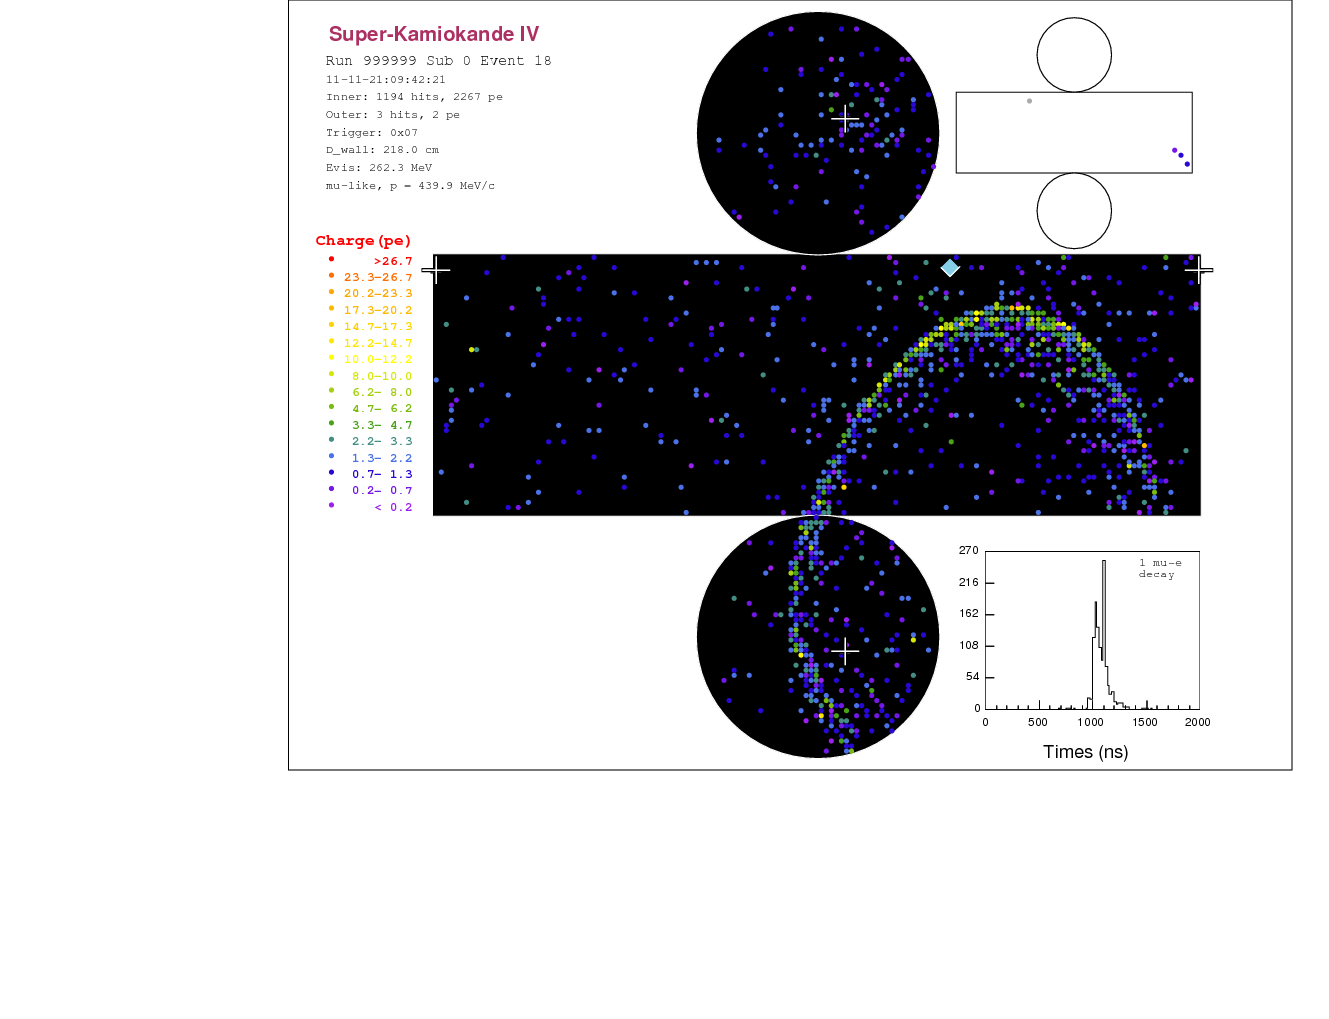
\includegraphics[width = \linewidth]{sk_mu} \\ (a)
  \end{minipage}
  \begin{minipage}{0.49\linewidth}
    \centering
    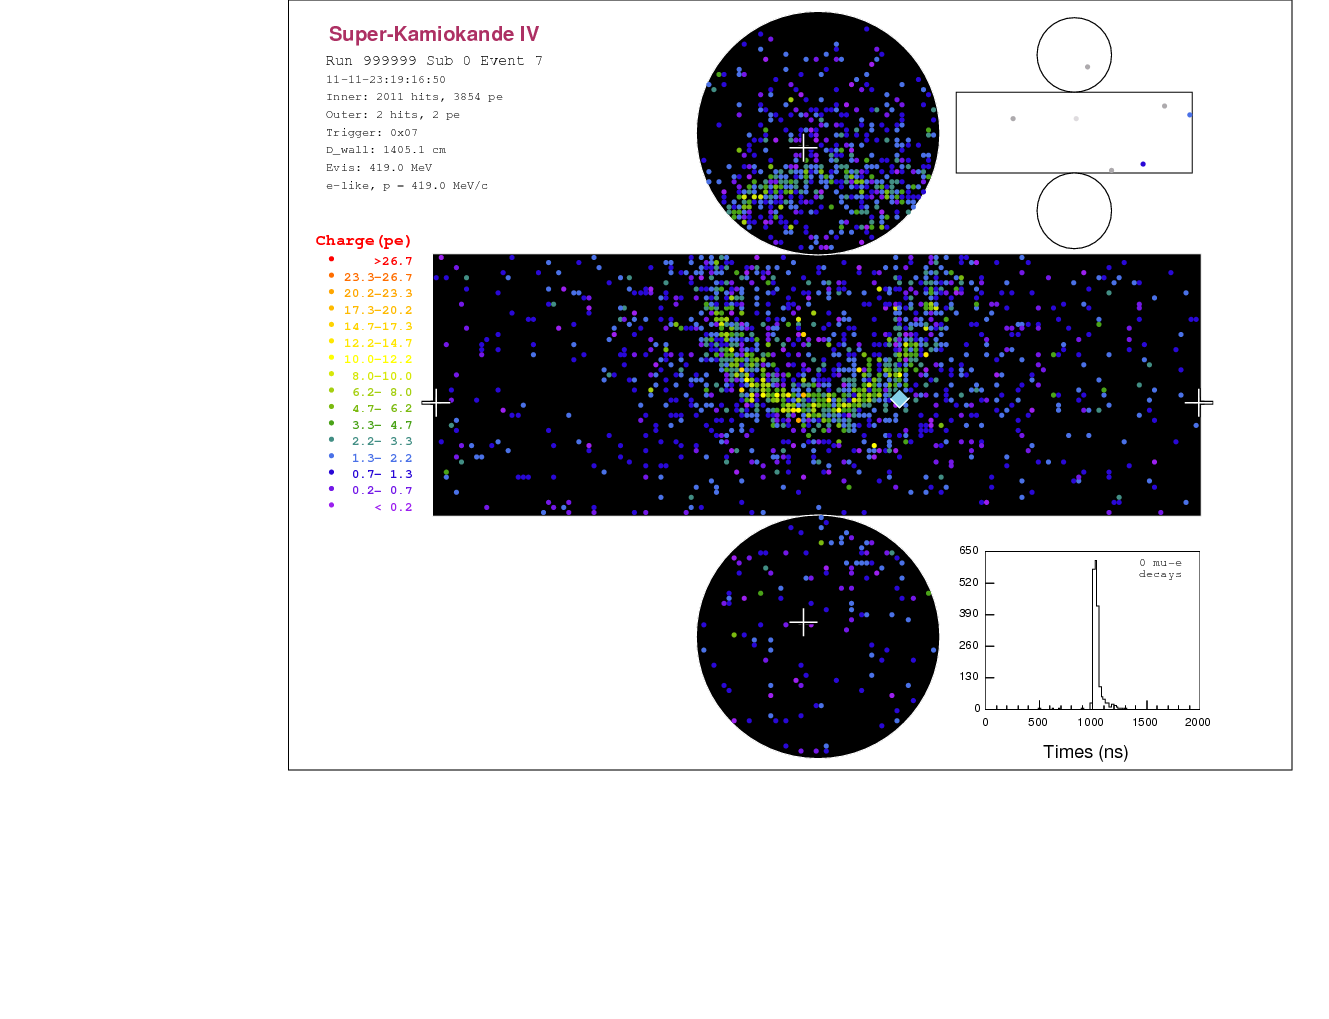
\includegraphics[width = \linewidth]{sk_e} \\ (b)
  \end{minipage}
    \caption{The event display of Cherenkov ring inside Super-Kamiokande detector: (a) ring from muon, (b) ring from electron.}
    \label{fig:T2K:sk_PID}
\end{figure}

The SuperKamiokande provides powerful shielding from the cosmic rays, but the atmospheric neutrino could easily go through the rock and interacts inside the inner detector. That's how the atmospheric studies are done, but for the T2K we need to distinguish neutrinos from the atmosphere and from J-PARC accelerator. The timing is the most useful information for this propose. As mentioned in the \autoref{ch:T2K:nu_beam} the beam is grouped in 8 bunches 19 ns width coming each 2 second. The time synchronization between J-PARC and Super-Kamiokande allow to select accurately neutrinos that fall into bunches and suppress the atmospheric background that is uniform in time. Thus the background is suppressed at the level of 8 orders.


\section{Analysis overview}
\subsection{Oscillation analysis}
As mentioned in the introduction the main goal of the T2K experiment is precise measurements of the neutrino oscillation parameters and search for the CP--violation. The scheme of the analysis workflow is presented in \autoref{fig:t2k:ana}. Different colors at the block-scheme represent the measurements (green), models (violet) and fit algorithms (blue).

\begin{figure}[ht!]
  \centering
  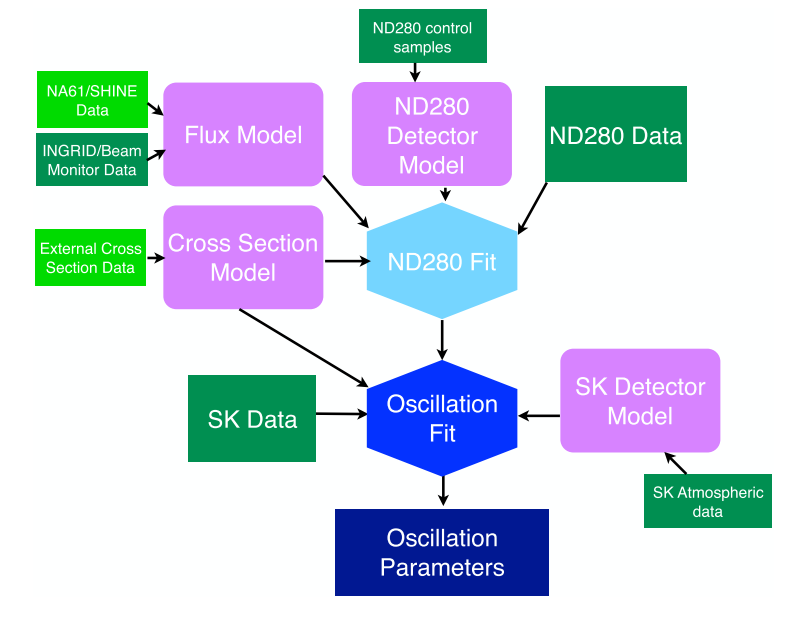
\includegraphics[width=0.8\linewidth]{t2k_ana_scheme}
  \caption{The scheme of the T2K oscillation analysis workflow. The measurements are presented in green (light --- external, dark --- T2K), the models are presented in violet and the fitter tools are presented in blue.}
  \label{fig:t2k:ana}
\end{figure}

The measurements start with the beamline monitors where the parameters of the proton beam are estimated. Then the data from the NA61 experiment is used to estimate the meson production in the target. The resulting neutrino beam intensity and direction are monitored with the near on-axis detector INGRID. All these results allow us to build the neutrino flux model.

The near detector ND280 performs the measurements of the off-axis neutrino flux. The observations are sampled in the neutrino sign and the reaction topology: quasi-elastic, pion production, deep inelastic. We use the results of other experiments as a prior estimation for the rate of neutrino interactions. But there are plenty of the parameters in the model that could be tuned precisely using all the samples collected in the ND280. Thus flux and the cross-section model are tuned together with the ND280 control samples.

The long history of the atmospheric neutrino measurements in Super-Kamiokande provides the accurate knowledge of the detector operation. This model is used together with the T2K events in thew SK for the final oscillation measurements. The spectrum of the observed electron neutrinos in the far detector is presented in \autoref{fig:t2k:nu_e}.

\begin{figure}[ht!]
  \centering
  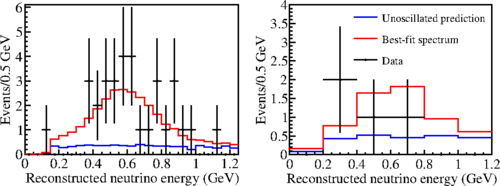
\includegraphics[width=0.9\linewidth]{nu_e}
  \caption{The spectrum of the electron neutrinos observed with the far detector comparing to the expectations without oscillation.}
  \label{fig:t2k:nu_e}
\end{figure}

As one could see the oscillation fit is a heart of the analysis. Three independent methods were developed for the fit machinery.
\begin{itemize}
  \item BANFF (Beam And ND280 Flux extrapolation task Force) is not an oscillation analysis tool, but it is a prefit method that use the data from both flux, near detector and cross-section models to constrain the initial parameters of the neutrino beam before the oscillations and precisely constrain the neutrino interactions model as well
  \item PiTheta analysis is based on the Poisson statistics and constrains the oscillation parameters with the likelihood minimization. It is using data binned in the lepton momentum and direction for the oscillation fit. This approach uses BANFF results and then fir the SK data to obtain the final result
  \item VaLOR (ValenciaLancaster-Oxford-Rutherford) is one more analysis using the minimization of the likelihood within Poisson statistics. It uses the samples binned in the neutrino energy and lepton direction
  \item MaCH3 (Markov CHain) approach is based on Bayesian statistics. Instead of using the near detector fit and propagating it to the far detector the both detectors' samples are fit together. The oscillation parameters are estimated with a Markov chain method. The data samples are binned in the neutrino energy and lepton direction
\end{itemize}

The result is considered as robust only if all the methods are in a good agreement about the confidence/creditable intervals. The oscillation results are presented in \autoref{fig:T2K:osc_res}.

\begin{figure}[h!]
  \centering
  \begin{minipage}{0.49\linewidth}
    \centering
    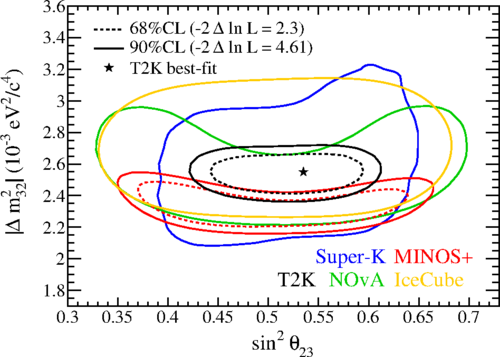
\includegraphics[width = \linewidth]{osc_res} \\ (a)
  \end{minipage}
  \begin{minipage}{0.49\linewidth}
    \centering
    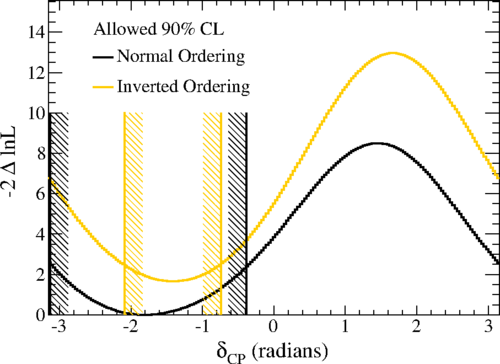
\includegraphics[width = \linewidth]{cp} \\ (b)
  \end{minipage}
    \caption{The oscillation results from the T2K experiment: (a) $\theta_{23}$ and $\Delta m_{32}^2$ constraints and (b) $\delta_{CP}$ constraints.}
    \label{fig:T2K:osc_res}
\end{figure}

\subsection{Neutrino cross-section measurements}
Alongside the oscillation analysis T2K performs very precise measurements of the neutrino cross-sections. The knowledge of the neutrino interactions' rates is essential for the oscillation analysis as the most realistic theoretical model could be chosen. The ND280 provides an opportunity to study neutrino interaction with carbon, oxygen and iron with both neutrino and anti-neutrino and with both flavors: muon and electron. The dominating sample in the ND280 is a muon neutrino interaction with no pions in the final state. For the T2K energies it's a main process that's why it's studied pretty well~\cite{Abe2020a}. Much more complicated analyzes are the interaction of the electron neutrinos. The result of the comparison of the $\nu_e$ and $\overline{\nu}_e$ cross-section is presented in \autoref{fig:t2k:nue_Xsec}~\cite{Abe2020}.

\begin{figure}[!ht]
  \centering
  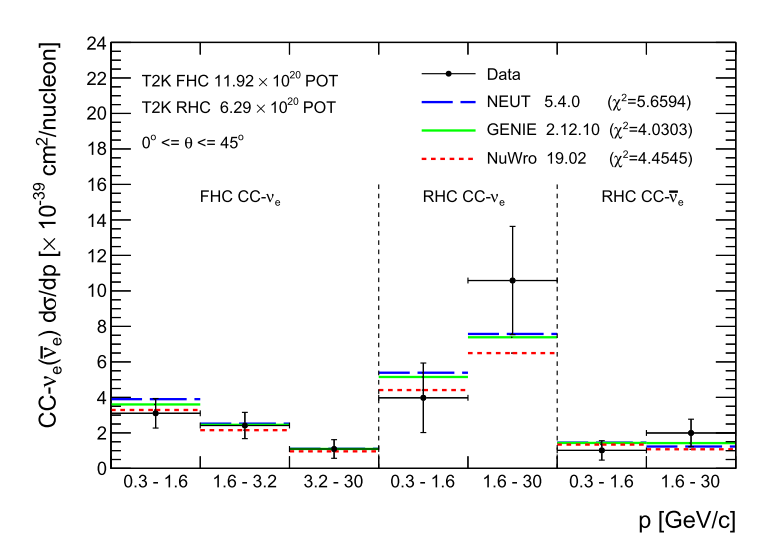
\includegraphics[width = 0.7\linewidth]{nue_Xsec}
  \caption{The result of the cross-section measurements in the ND280. Results for $\nu_e$ and $\overline{\nu}_e$ are compared against various theoretical models.}
  \label{fig:t2k:nue_Xsec}
\end{figure}

\end{document}